\documentclass[12pt]{ujreport}
\usepackage[dvipdfmx]{graphicx}

\usepackage[bachelor]{AIcover}	% 卒論の場合
%\usepackage[master]{AIcover}		% 修論の場合
\usepackage[dvipdfmx]{graphicx}
\usepackage{AIthesis}
\usepackage{geometry}
\usepackage{setspace}
\usepackage{listings}
\usepackage{subfigure}
\usepackage{caption}

%\setlength\intextsep{0pt}
%\setlength\textfloatsep{0pt}
%\makeletter
%\newcommand{figcaption}[1]{def\@captype{figure}\caption{#1}}
%\newcommand{tblcaption}[1]{\def\@captype{table}\caption{#1}}
\renewcommand{\bibname}{参考文献}
\input personal

\begin{document}
\makeCoverPageII
\newpage

\newgeometry{margin=0mm}
\begin{figure}
  \centering
  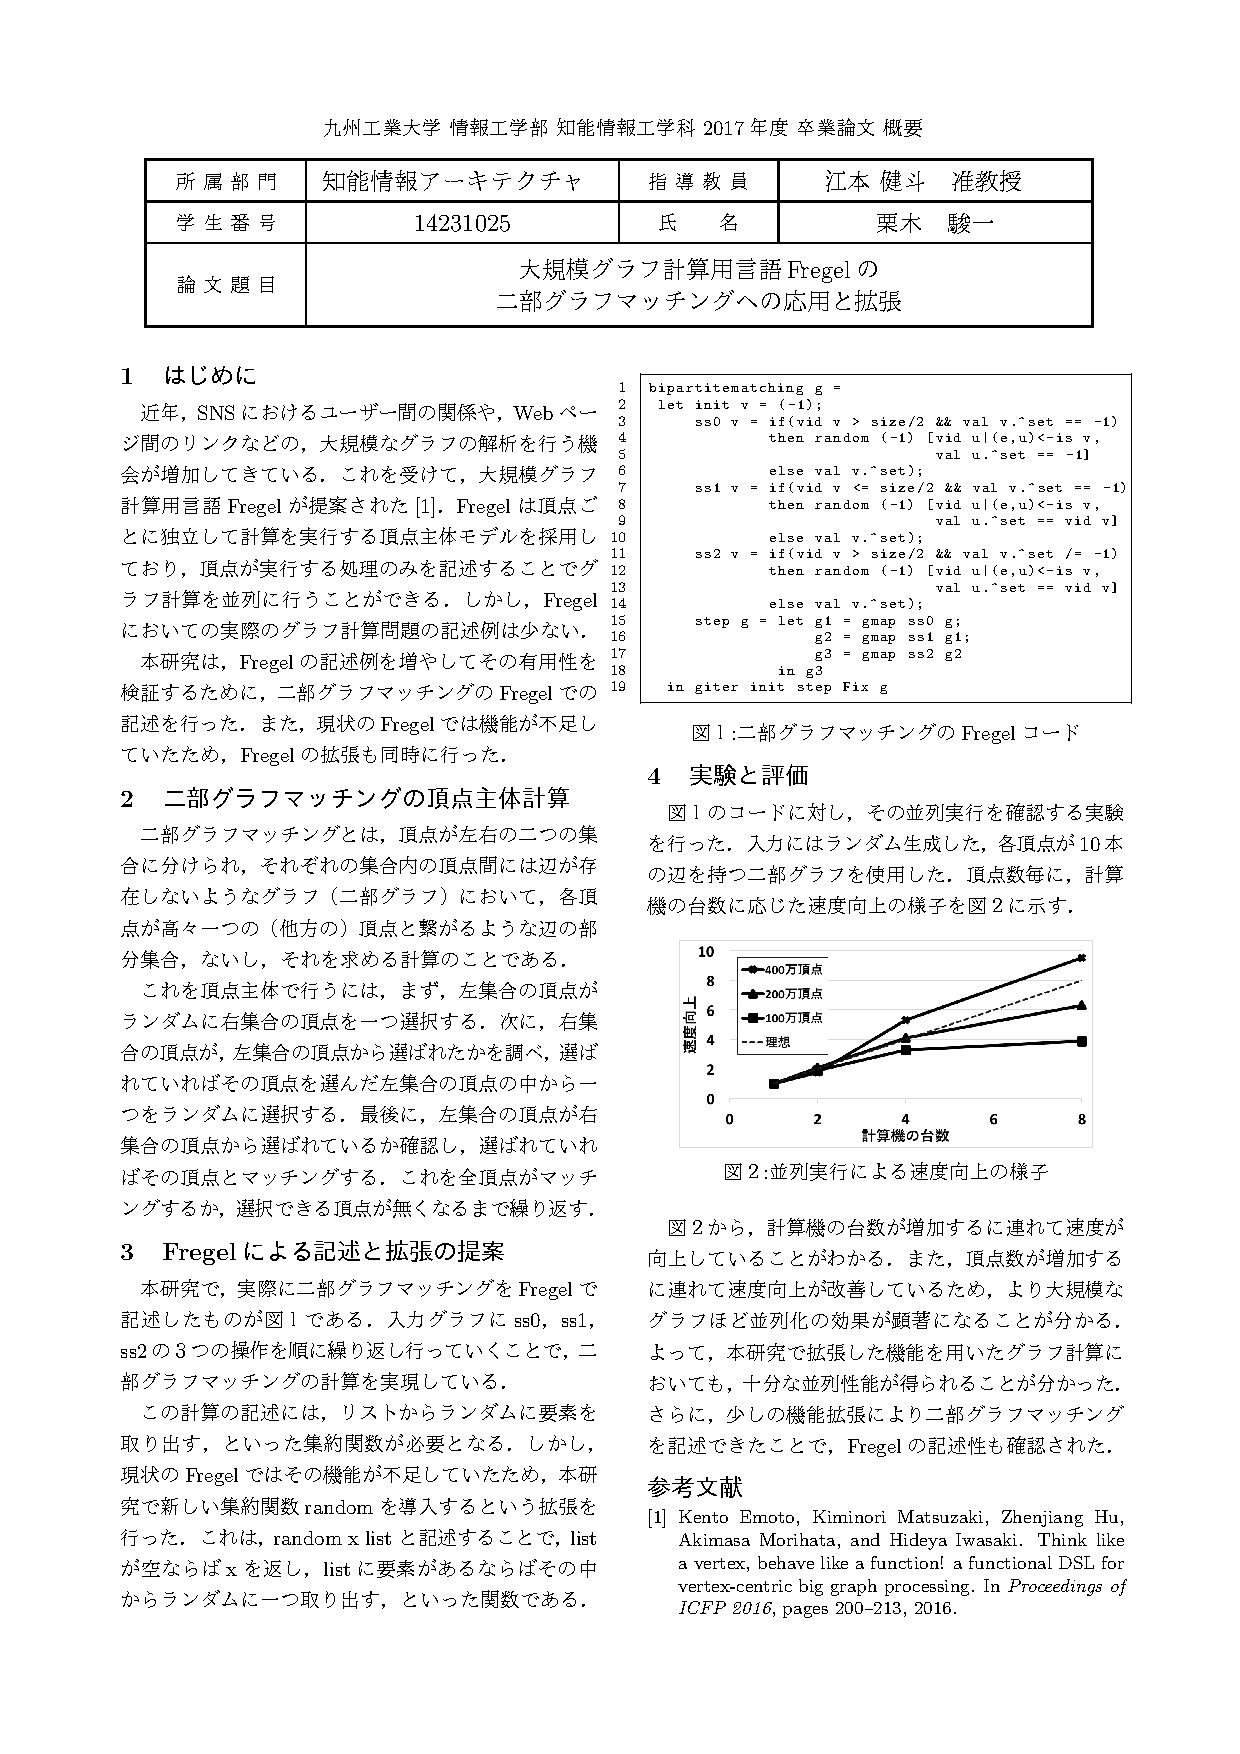
\includegraphics[width=21.0cm]{abst.pdf}
\end{figure}

\restoregeometry

\pagestyle{plain}
% 目次
\pagenumbering{roman}	%目次のページ番号(ローマ字)
\tableofcontents 		%目次作成
\newpage
\pagenumbering{arabic} 	%本編ページ番号

\chapter{はじめに}
近年,SNSにおけるユーザー間の関係や,Webページ間のリンクなどの,大規模なグラフの解析を行う機会が増加してきている.
例えば,SNSのユーザーを頂点,ユーザー間のフォロー/フォロワー関係を辺とすると,SNSは大規模なグラフと考えることができる.
このグラフに対して解析を行うことで,そのユーザーに関係のあるユーザーを提示したり,ユーザーが興味を示す情報を提示することができる.
このような大規模グラフを扱う計算を実行しようとすると,単一の計算機では時間がかかるため,複数の計算機を用いて並列処理を行う必要がある.

そこで,大規模グラフを並列処理するためのフレームワークとしてPregel \cite{pregel}が提案されている.
Pregelは頂点主体の計算モデルを採用しており,ユーザーは各頂点で繰り返される単一の計算を記述するだけで,グラフ計算を並列に行うことができる.
しかし,Pregelの問題点として,複雑なアルゴリズムを記述する場合にはプログラミングが難しい,ということが挙げられている.
この問題点を解決するためにPregelモデルを高階関数として定式化し,関数型の領域特化言語として実現したFregel \cite{fregel}が提案された.
Fregelで記述されたプログラムはPregelに変換することができ,現在はPregelのオープンソース実装であるApache Giraphへのコンパイラが用意されている.
しかし,このFregelでのグラフ計算問題の記述例はまだまだ数が少ない.

本研究は,Fregelの記述例を増やし,その有用性を検証するために,二部グラフマッチングのFregelでの記述を行った.
また,現状のFregelではこのグラフ計算を実現するための機能が不足していたため,Fregelの機能の拡張を行った.
拡張した機能を用いて二部グラフマッチングを記述し,並列実行により実験を行なった結果,十分な並列性能を確認することができた.

以降の論文の構成について述べる.
2章では,本研究で利用するPregelやFregelについて説明する.
3章では,二部グラフマッチングについてと,Pregelによる二部グラフマッチングのアルゴリズムについて述べる.
4章では,Fregelによる二部グラフマッチングの記述と,それに必要となったFregelの拡張の提案を行う.
5章では,実際に大規模なグラフで二部グラフマッチングを並列実行した実験の結果を述べる.
6章では,本研究についてまとめる.

\newpage

\chapter{準備}
\section{Pregel}
Pregel \cite{pregel}はGoogleが提唱した大規模グラフを並列処理するためのフレームワークである.
Bulk Synchronous Parallel(BSP)に基づく頂点主体の計算モデルを提供している.
このモデルでは,ユーザーは各頂点の振る舞い(頂点計算)を記述するだけでグラフ計算のための並列プログラムを作ることができる.

\subsection{概要}
Pregelでは,各頂点がユーザーの記述した同一の処理を実行すること(superstep)と,
全ての頂点での処理の終了を待つこと(バリア同期)の繰り返しによってグラフ計算が実行される.
この繰り返しは,グラフ計算が収束するまで実行される.
また,頂点での処理実行は全頂点で並列に実行される.

\subsection{メッセージの送受信}
頂点間の通信はメッセージの送受信によって行われる.
superstep Sの処理を実行する時,頂点は一つ前のsuperstep S-1の処理にて送信されたメッセージを参照することができる.
またsuperstep Sの処理で送信されたメッセージは次のsuperstep S+1で利用することができる.
このように頂点が送信したメッセージは次のsuperstepでのみアクセスできる,といった制限を設けることで通信によるデッドロックを回避することができる.
これはある頂点が必要とするメッセージはバリア同期によって送信されていることが保証されているからである.
メッセージの送信は頂点IDに基づいて行われるが,基本的にメッセージの送信はその頂点の隣接点への送信である.

\subsection{計算の終了判定}
Pregelの計算はsuperstepとバリア同期の繰り返しで,全ての頂点での計算が収束(終了)するまで繰り返される.
その収束を判定するため,各頂点はActiveとInactiveという二つの状態を持つ.
全ての頂点がInactiveになることでグラフ全体の計算を終了する.
Activeな頂点はユーザーの記述した処理を実行し,Inactiveな頂点は実行しない.
処理の中でvoteToHaltと呼ばれる操作が行われると,その頂点の状態がActiveからInactiveへ変化する.
またInactiveな頂点はメッセージを受信することでActive状態となる.

\subsection{Pregelでの計算例}
Pregelでの計算の例として,ある頂点から到達可能な頂点を調べる到達可能性問題のコードをListing 2.1に示す.
このプログラムは有向グラフを入力とする.
頂点と受信メッセージを入力として受け取り,始点から到達可能(true)とマークされた頂点の隣接頂点をtrueとマークしていく.
このコードは主に初期化部分(2-5行目)と繰り返しの部分(6-10行目)に分けることができる.

最初のsuperstepでは,計算を実行している頂点(v)が始点かどうか判別し,始点ならばtrueとマークしその情報を隣接頂点へ送信する.
以降のsuperstepでは,受信したメッセージにtrueが含まれていて,かつ,まだ自身がfalseであるならば,自身をtrueとマークしてそのことを隣接頂点へ伝える.
最後にvoteTohaltによって頂点をInactiveにする.
\begin{lstlisting}[basicstyle=\ttfamily\footnotesize, frame = single,  numbers = left, tabsize = 3, captionpos = b, caption = {Pregelのプログラム例}]
vertex.compute(v,message){
  if(superstep == 0){
    v.rch = v.vid == 0;
    if(v.rch)
      sendToNeighbors(v.rch);
  }else{
    newrch = v.rch || or(message);
    if(newrch != v.rch){
      v.rch = newrch;
      sendToNeighbors(newrch);
    }
  }
  voteToHalt();
}
\end{lstlisting}

図2.1にPregelモデルを用いた到達可能性問題を解く過程のグラフを示す.
左が入力グラフであり,残りの右のグラフは表示されている回数のsuperstep終了後のグラフを表している.
白の頂点はActiveな状態,灰色の頂点はInactiveな状態であることを示す.

初めに,superstep0では始点である頂点にtrueがマークされ,隣接している2つの頂点へtrue(T)のメッセージが送信される.
superstep1ではメッセージを受信した2つの頂点はactive状態となり,始点はInactiveとなる.
tureのメッセージを受信した頂点はtureをマークし,隣接している頂点へtureを送信する.
superstep2で最後の頂点にtrueがマークされる.
superstep3で全ての頂点がInactiveの状態になるため計算が終了する.

\begin{figure}[ht]
  \centering
  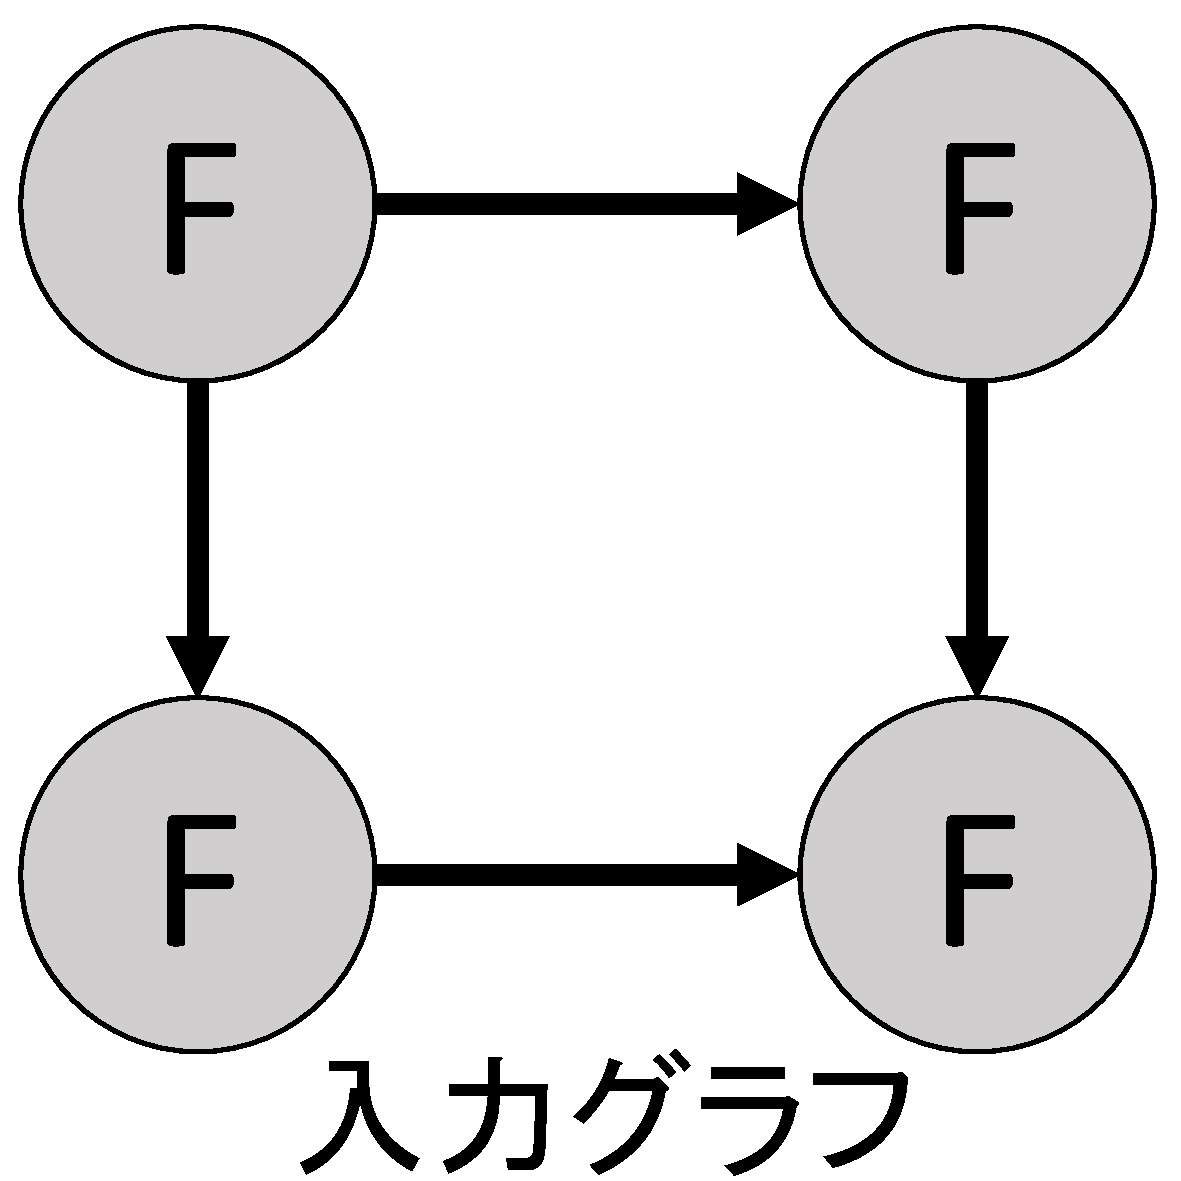
\includegraphics[width=2.5cm]{入力.pdf}
  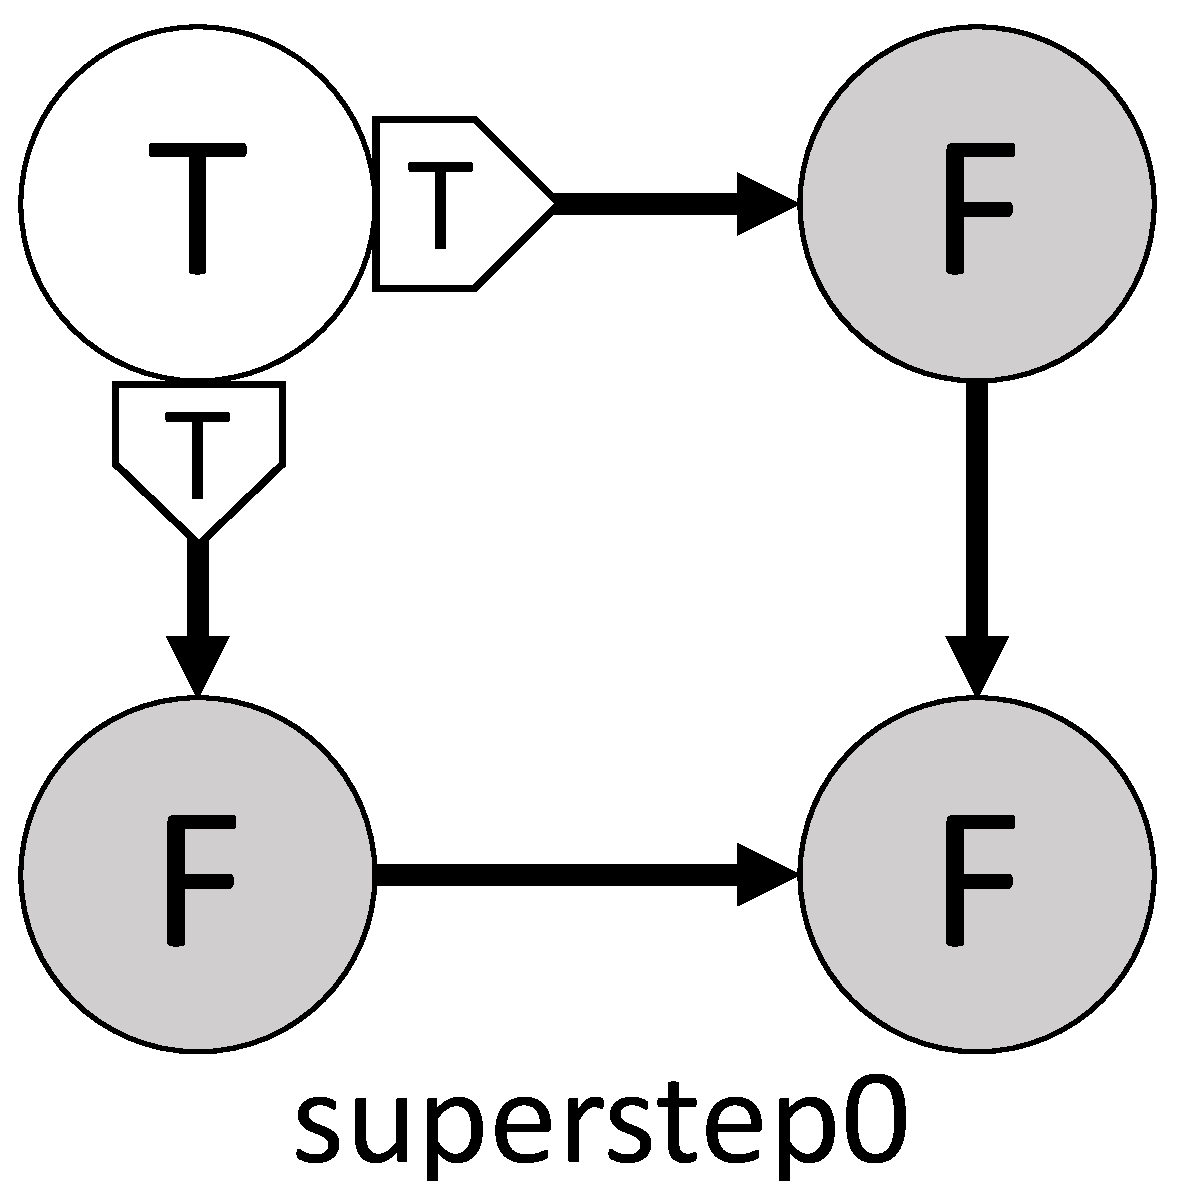
\includegraphics[width=2.5cm]{ss0.pdf}
  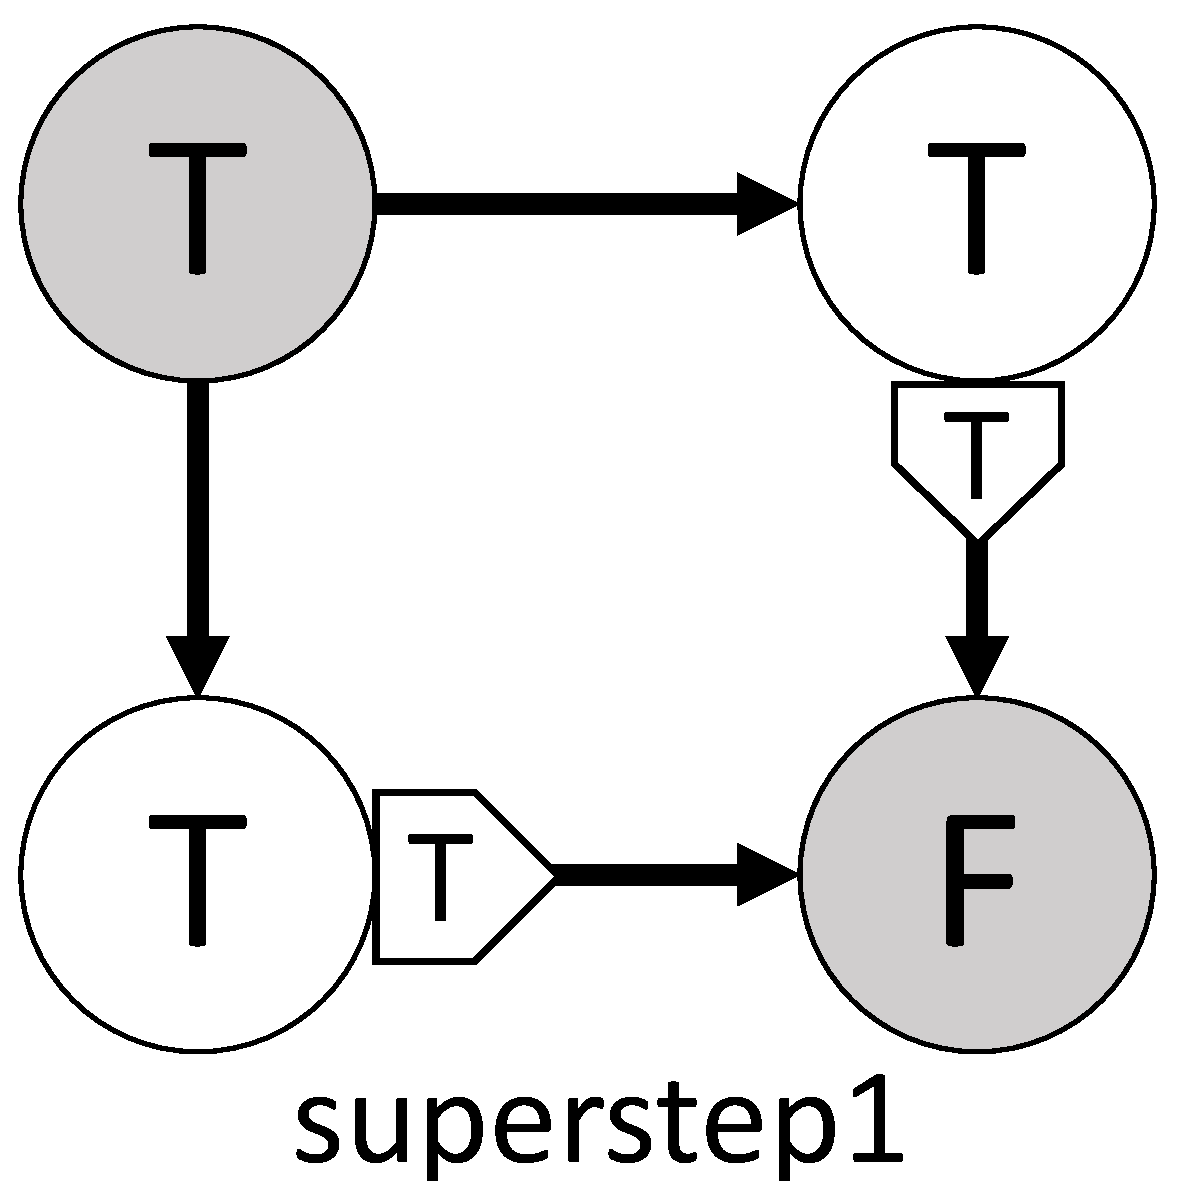
\includegraphics[width=2.5cm]{ss1.pdf}
  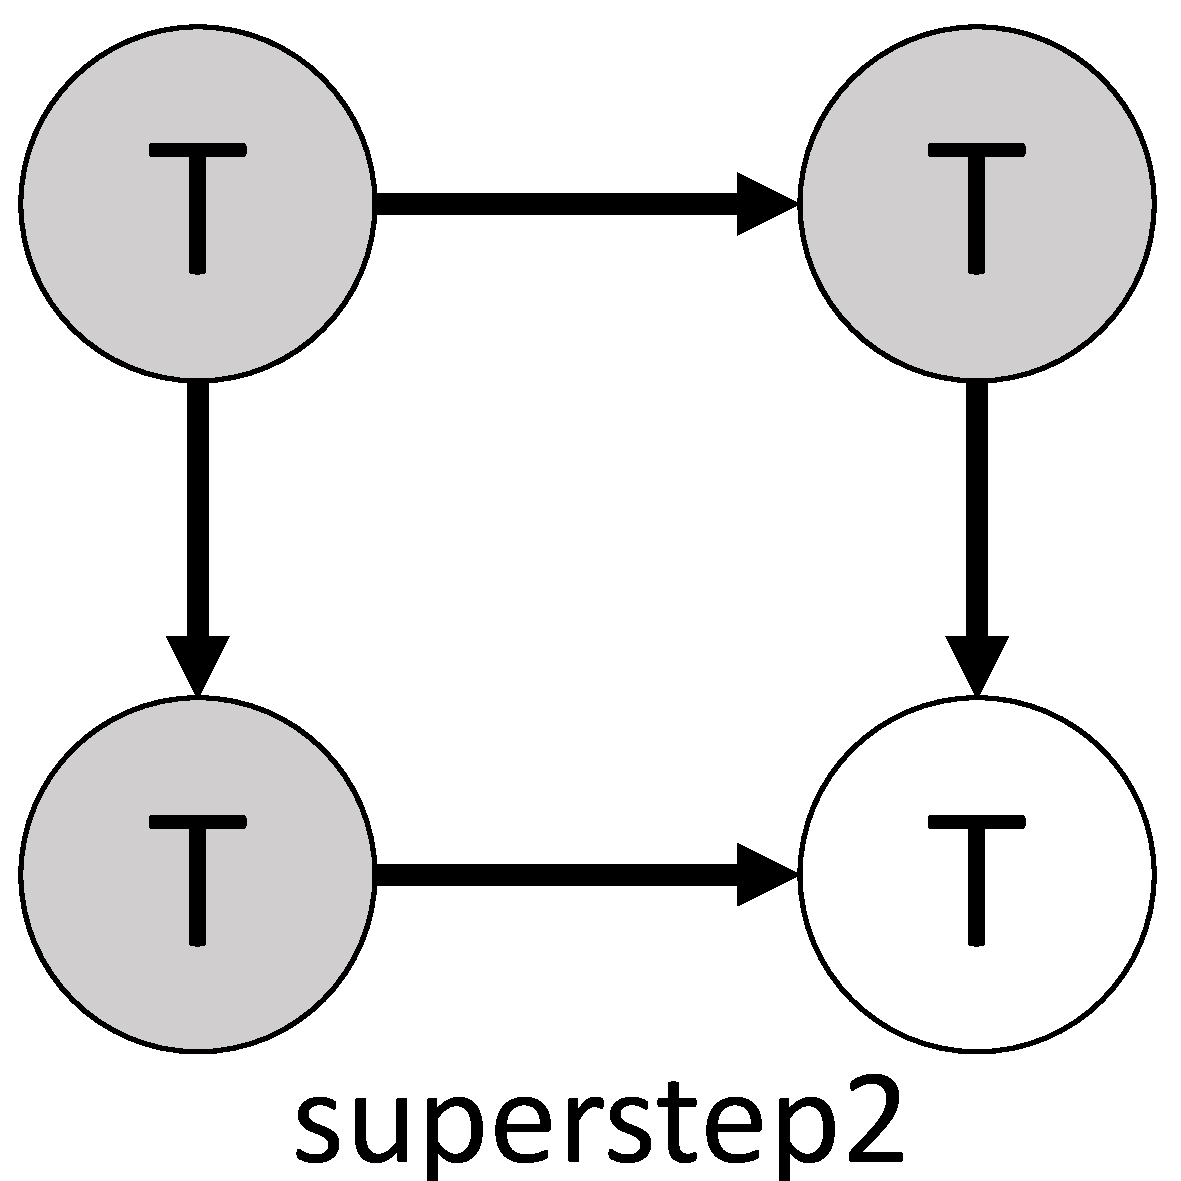
\includegraphics[width=2.5cm]{ss2.pdf}
  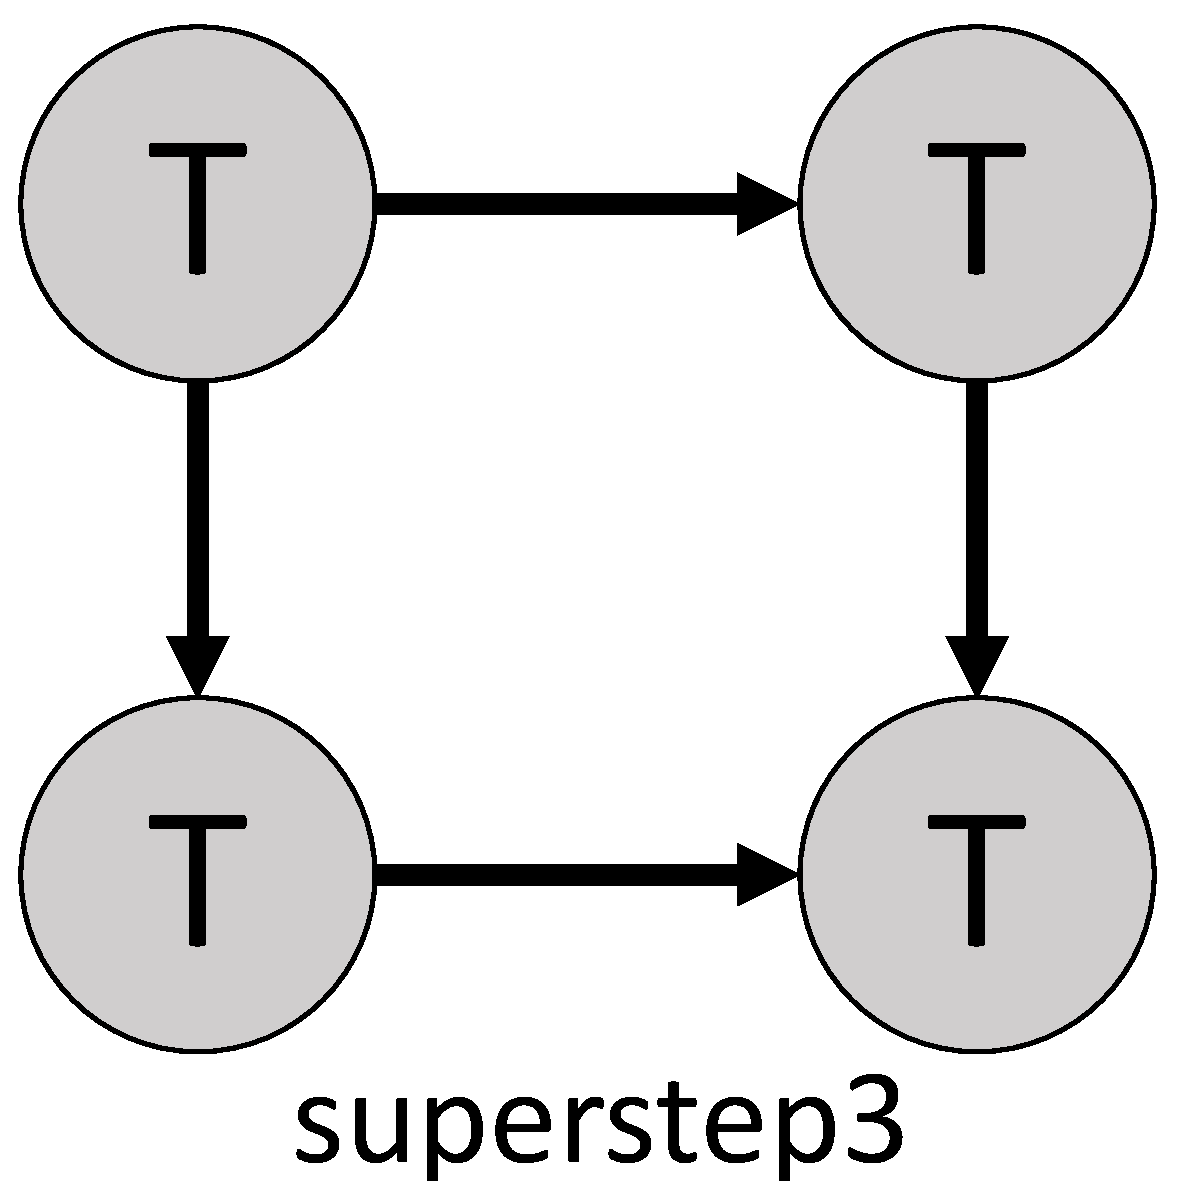
\includegraphics[width=2.5cm]{ss3.pdf}
\caption{Pregelの計算過程の様子}
\end{figure}

\subsection{Pregelの問題点}
Pregelプログラミングは採用しているBSPモデルの通信に関する制約から,任意のグラフ計算を必ずしも簡単に書けるものではない.
これには,主に3点の理由が挙げられる.

まず1つ目に,明示的な状態制御の難しさである.隣接した頂点や全頂点,グラフ全体の情報を集約し,その情報を用いて計算を行いたい場合がある.
その場合,異なるsuperstepで異なる振る舞いをするように,superstepの回数で判定するなどして状態の制御を明示的に行われなければならない.

2つ目に,明示的なメッセージの送受信の問題がある.
頂点間の通信はメッセージの送受信によって行われるが,そのsuperstepで使いたい情報は1つ前のsuperstepで送信しなければならない.
複雑なプログラムになってくるとメッセージを送信する箇所,受信したメッセージを使用する箇所などを明確に把握していく必要がある.
そのため,複雑なプログラムになるにつれてメッセージのやり取りや制御の流れの把握が困難になる問題点が挙げられる.

最後に,3つ目の問題点として明示的な計算停止制御が挙げられる.
Pregelでは計算を終了させるために各頂点の処理として,voteToHaltを呼び出す必要がある.
したがって,全頂点の計算を適切に終了させるためには各頂点における処理を正しく記述する必要がある.
しかし,複雑なプログラムになるにつれて正しく処理を追うことが困難になってくる.
そのため,予期せぬところで計算が停止したり,voteToHalt操作が正しく呼び出されず計算が止まらないなど,適切な場面で計算を終了させることが困難になってくる.

\section{Fregel}
Fregel \cite{fregel}とは,Pregelの問題点を解決しようと提案された,大規模グラフ処理のための関数型領域特化言語である.

\subsection{概要}
FregelはPregelモデルを基本に設計されている.
Haskellプログラムとして動作可能であり,Haskellインタプリタを用いた動作確認やデバックが可能となっている.
また,高階関数を用いたグラフ計算の記述が可能となっており,この高階関数はひとつのFregelプログラムの中で複数回使用することができる.
Pregelでは頂点間の通信の表現としてpoke-baseの通信の表現を採用していたが,Fregelではpeek-baseの通信の表現を採用している.
これにより,頂点間での必要な情報のやり取りを,より直感的に記述することができるようになっている.

\subsection{Fregelにおける通信の表現}
Fregelでは,peek-baseの通信の表現を用いることで,Pregelの問題点として挙げた明示的なメッセージの送受信の問題を解決している.
Pregelにおけるpoke-base,Fregelにおけるpeek-baseの通信の表現を図2.2に示す.
頂点vでの頂点計算を行う場合に,隣接している頂点uの情報を使用したい場合を考える.
Pregelにおけるpoke-baseの通信では使用したい頂点uの情報を頂点vへ送信するように記述する必要がある(例:Listing 2.1の10行目).
しかし,Fregelにおけるpeek-baseの通信では,頂点vが使いたい頂点uの情報を自分から見に行く,といった振る舞いになるため明示的な通信の記述をする必要がない(2.2.5節で例示する).

\begin{figure}[ht]
  \centering
  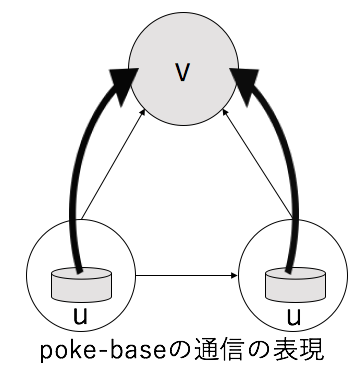
\includegraphics[width=4cm]{pokebase.png}
  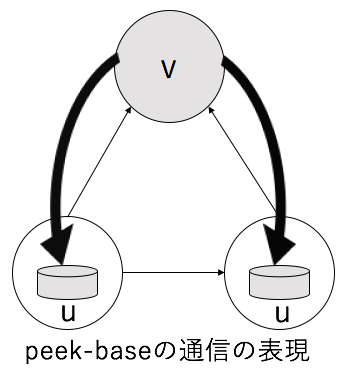
\includegraphics[width=4cm]{peekbase.png}
\caption{通信の表現}
\end{figure}

\subsection{グラフ高階関数}
Fregelは様々なグラフ処理を簡単に記述するために次の4つの高階関数を提供している.
関数fregelはPregelの関数的モデルを実装し,初期化関数,ステップ関数,終了条件を受け取る.
関数gzipは2つのグラフを受け取り,対応する頂点をペアとする.
関数gmapはグラフの全頂点に与えられた関数を適用する.
関数giterは関数fregelと同様に初期化関数,ステップ関数,終了条件を受け取る.
この関数はグラフを受け取り,そのグラフに処理を適用した後のグラフを返すものである.
そして受け取った終了条件が満たされるまで繰り返し関数の適用を繰り返す.

\subsection{終了条件}
高階関数fregel,giterが受け取る終了条件としてFix,Until,Iterの3つが用意されている.Fixはグラフの各頂点の値が変化しなくなる不動点に達するまで計算を行う.
Untilは式を引数として受け取り,その式が満たされるまで計算を実行する.Iterは整数を引数として受け取り,その回数分計算を実行する.

\subsection{Fregelでの計算例}
例としてListing 2.2に到達可能性問題のFregelプログラムを示す.
1行目では頂点が持つデータ型を定義している.
そして,2行目以降の関数reAllが主要な部分となる.
init部分が初期化関数にあたり,その頂点が始点である場合のみrchフィールドの値がTrueであるRvalレコードを返す.
頂点のIDは特殊なプリミティブ関数vidで取得している.
ステップ関数stepは直前のrchフィールドに格納されている結果を隣接頂点から集約している.
これはis vを生成子とする内包表記で実現している.
この結果と自分の値の論理和をor関数で求めることで,隣接している頂点が到達可能ならば自身も到達可能であるとマークすることができる.
7行目は高階関数fregelの引数が上で定義した初期化関数init,ステップ関数step,終了条件のFix,グラフgとなっている.

\begin{lstlisting}[basicstyle=\ttfamily\footnotesize, frame = single,  numbers = left, tabsize = 3, captionpos = b, caption = {Fregelのプログラム例}]
data Rval = Rval { rch :: Bool } deriving Eq
 reAll g =
   let init v = Rval(vid v == 0)
       step v prev curr =
        let newrch = prev v.^rch||or [prev u.^rch | (e,u) <- is v]
       in Rval newrch
   in fregel init step Fix g
\end{lstlisting}

\section{Apache Giraph}
Apache Giraph \cite{giraph}とは,オープンソースのフレームワークで,Apache Hadoop~\cite{hadoop}と呼ばれる分散処理環境で実行されるシステムである.
Java言語により実装されており,GiraphプログラムもJava言語を使って記述する.本研究の実験ではFregelで作成したコードをGiraphにコンパイルし,動作させる.

\newpage

\chapter{二部グラフマッチングの頂点主体計算}
\section{二部グラフマッチング}
二部グラフとは,図3.1のような,頂点の集合が左右の二つの部分集合に分けられ,それぞれの集合内での頂点間には辺が存在しないようなグラフのことである.
グラフのマッチングとは,各頂点が高々一つの頂点と繋がるような辺の部分集合,ないし,それを求める計算のことである.

二部グラフマッチングは二部グラフにマッチングを適用したもので,図3.2の太くなっている辺が例として挙げられる.
マッチングは一つのグラフにおいて何通りか存在する場合もある.
本研究で扱うアルゴリズム \cite{pregel}は,必ずしも最大数のマッチングを得ることができないが,ある程度の大きさのマッチング数を確保するものとなっている.

\begin{figure}[ht]
  \centering
  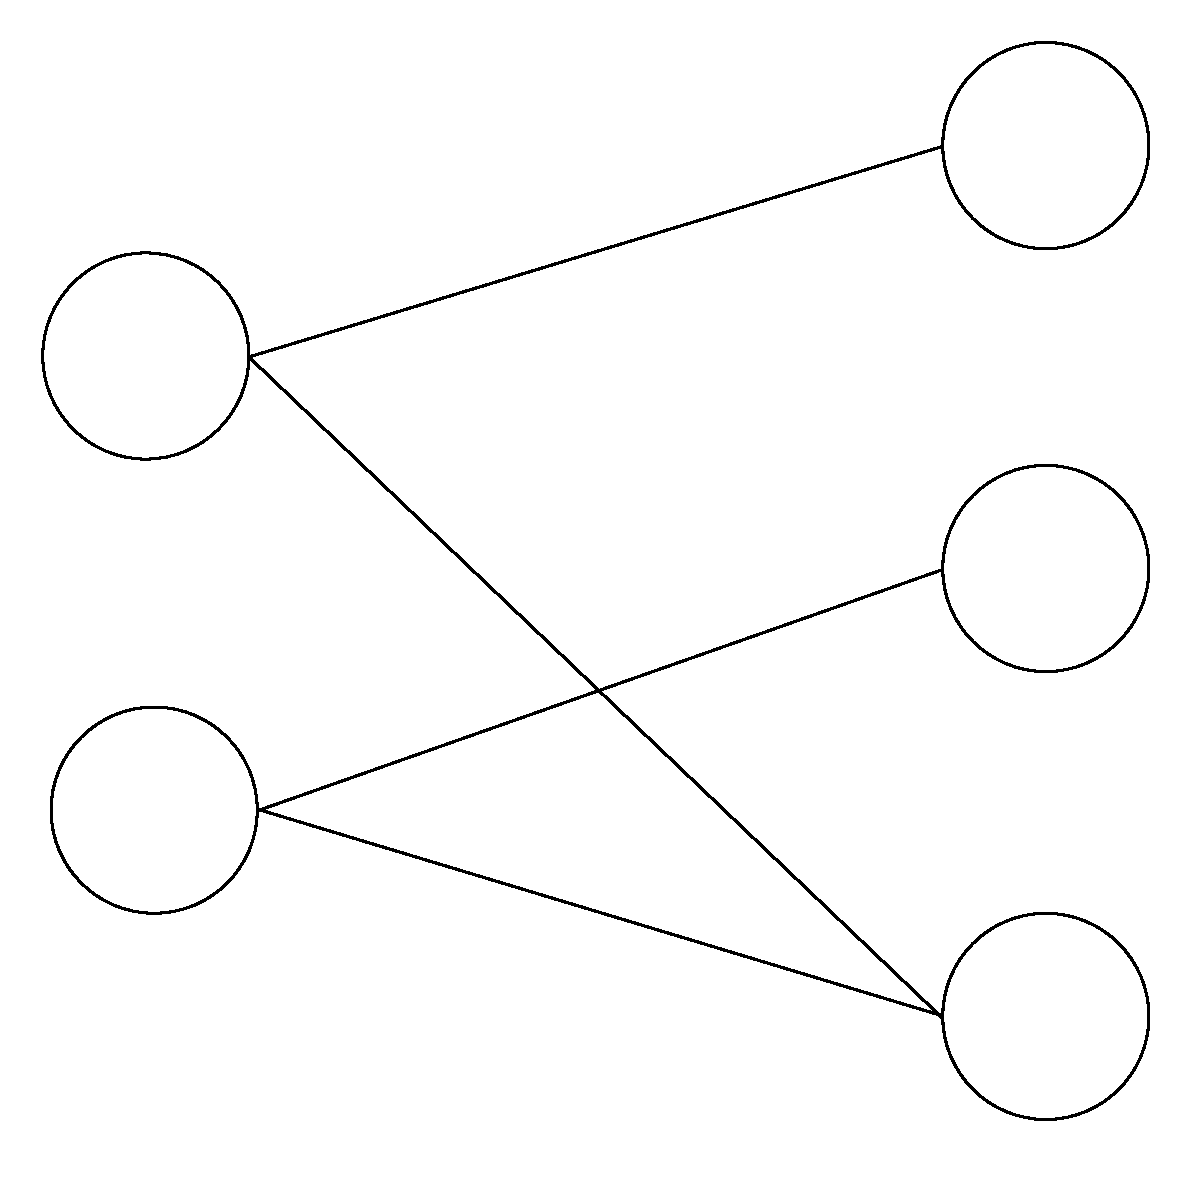
\includegraphics[width=6cm]{二部グラフ例.pdf}
  \caption{二部グラフの例}
\end{figure}

\begin{figure}[ht]
  \centering
  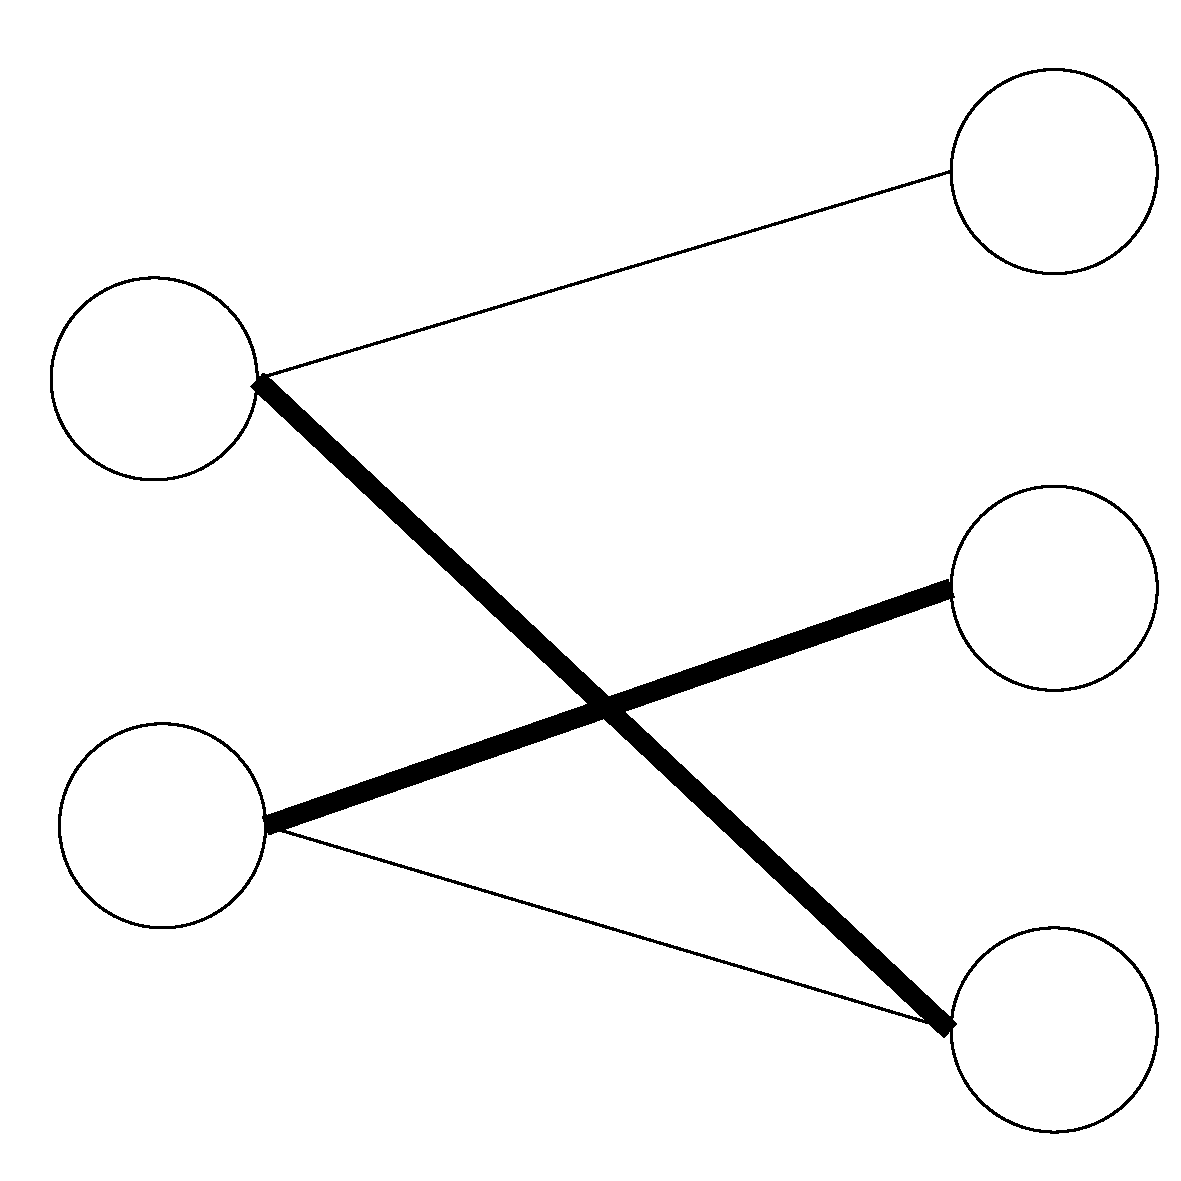
\includegraphics[width=5cm]{二部グラフ例1.pdf}
  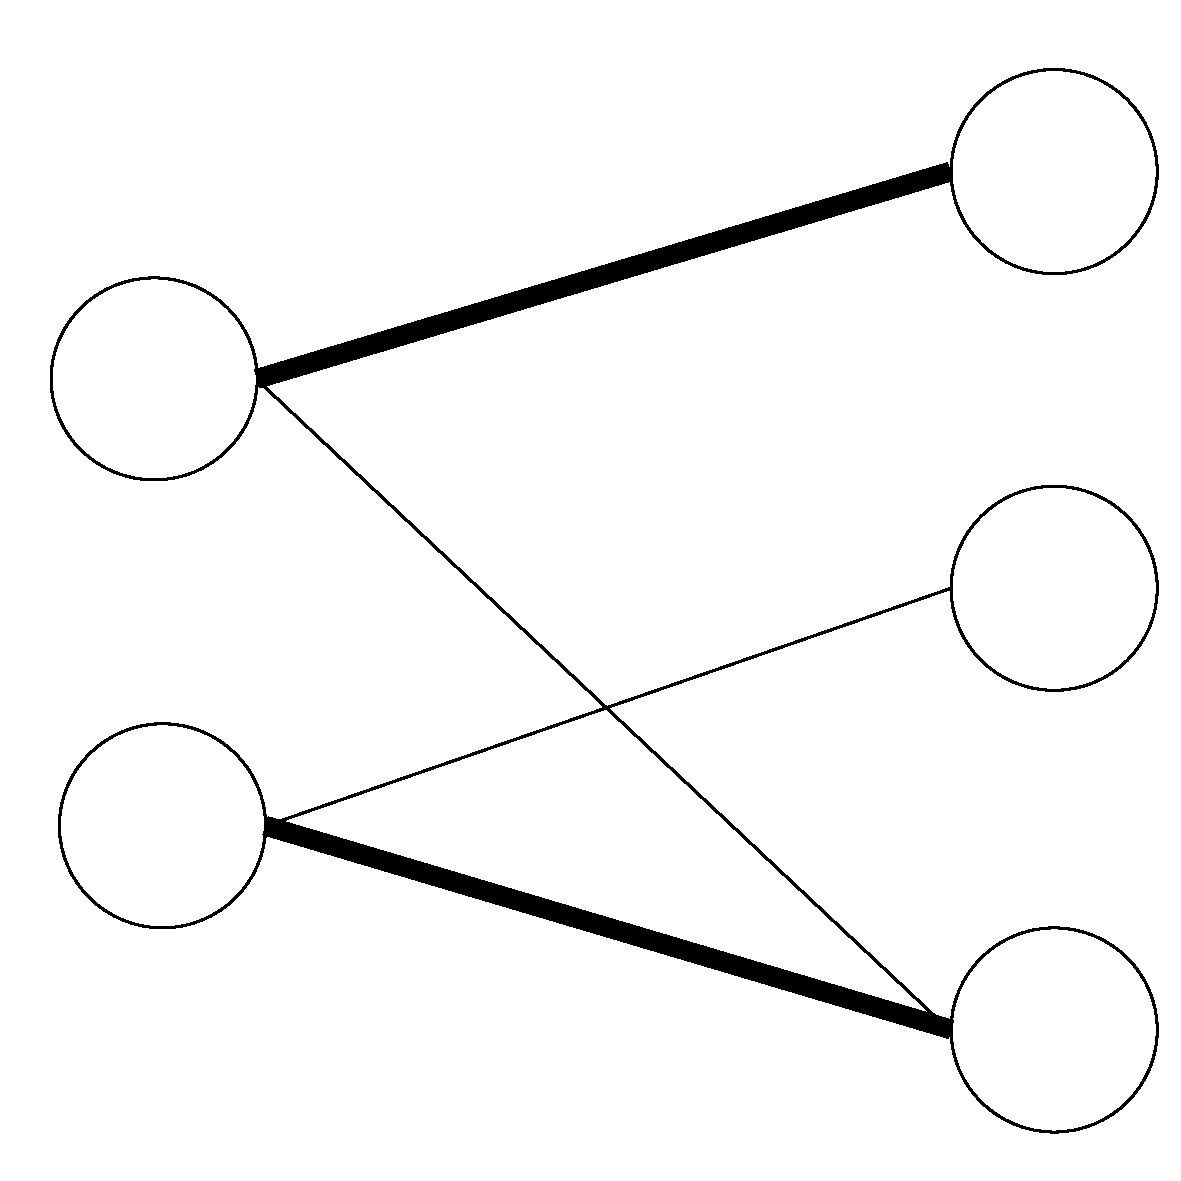
\includegraphics[width=5cm]{二部グラフ例2.pdf}
\caption{二部グラフマッチングの例}
\end{figure}

\section{Pregelアルゴリズム}
二部グラフマッチングをPregelで記述したものがListing3.1である.
このアルゴリズムは4回のsuperstepを1サイクルと考え,全頂点がマッチングするかマッチングできる頂点が無くなるまでサイクルを繰り返す.
各頂点は,自身のマッチング先の頂点IDを保持するものとなっている.

superstep0で,自身が保持しているマッチング先のIDの初期化として-1を入れる(4-6行目).
サイクル内の0番目でのsuperstep(case0)では,片方の集合の各頂点が,隣接している頂点全てにメッセージとして自分の頂点IDを送信する(6-12行目).
次のsuperstep(case1)では,他方の集合の各頂点が受け取ったメッセージからランダムに一つ選び,選んだ頂点IDにメッセージとして自分の頂点IDを,選ばななかった頂点IDに-1を送信している(13-40行目).
そして,その次のsuperstep(case2)では,まず,受け取ったメッセージの正負を確認する.
正であればメッセージの値を自分の値に代入し,その頂点IDへメッセージとして自分の頂点IDを送信する.
負であれば,選ばれなかったということなので値は-1のままにし,次のサイクルで再度マッチングを探す.
もし正の値であるメッセージが複数存在した場合は,その中からランダムに一つ選ぶようにする(41-62行目).
サイクル内最後のsuperstep(case3)で,受け取ったメッセージを自分の値に代入して1サイクルが終了となる(63-73行目).
次のサイクルが終わっても値が前のサイクルの値のままであれば,それ以上マッチングは存在しないということなので全体の計算が終了となる.

\newpage

\begin{lstlisting}[basicstyle=\ttfamily\scriptsize, frame = single,  numbers = left, tabsize = 3, captionpos = b, caption = {Pregelの二部グラフマッチング}]
public void compute(
  if(getSuperstep() == 0){
    vertex.setValue(new DoubleWritable(-1));
  }
  switch((int)getSuperstep() % 4) {
  case 0:
    if(vertex.getId().get()%2 == 0 && vertex.getValue().get() < 0) {
      double id = vertex.getId().get();
      sendMessageToAllEdges(vertex,new DoubleWritable(id));
      vertex.voteToHalt();
    }
    break;
  case 1:
    if(vertex.getId().get()%2 == 1 && vertex.getValue().get() < 0) {
      int mscount = 0,i = 0;
      double ms = 0;
      double id = vertex.getId().get();

      for(DoubleWritable message : messages) {
        mscount++;
      }
      if(mscount != 0){
        Random rnd = new Random();
        int rand = rnd.nextInt(mscount);

        for(DoubleWritable message : messages) {
          if(i == rand) {
            ms = message.get();
            sendMessage(new LongWritable((long)ms),new DoubleWritable(id));
          }
          else{
            ms = message.get();
            sendMessage(new LongWritable((long)ms),new DoubleWritable(-1));
          }
            i++;
          }
      }
    }
    vertex.voteToHalt();
    break;
  case 2:
    if(vertex.getId().get()%2 == 0 && vertex.getValue().get() < 0) {
      int mscount = 0,i = 0;
      long ms = 0;
      double id = vertex.getId().get();
      ArrayList<Long> mstrue = new ArrayList<Long>();
      for(DoubleWritable message : messages) {
        ms = (long)message.get();
        if(ms >= 0){
          mstrue.add(ms);
          mscount++;
        }
      }
      if(mscount != 0) {
        Random rnd = new Random();
        int rand = rnd.nextInt(mscount);
        sendMessage(new LongWritable(mstrue.get(rand)),new DoubleWritable(id));
        vertex.setValue(new DoubleWritable((double)mstrue.get(rand)));
        vertex.voteToHalt();
      }
    }
    break;
  case 3:
    if(vertex.getId().get()%2 == 1 && vertex.getValue().get() < 0) {
      double ms = vertex.getValue().get();
      for(DoubleWritable message : messages) {
        ms = message.get();
      }
      vertex.setValue(new DoubleWritable(ms));
      vertex.voteToHalt();
    }
    break;
}
\end{lstlisting}

Listing3.1のPregelの記述例では,頂点の実行する処理がcase毎に分割されている.
メッセージの送信部分や送信されたメッセージを使用している部分がcaseを跨いでいるため,どのメッセージを送信しているのか,どのメッセージを使用したいのか正確に把握しながら記述していく必要がある.
こういった点が第2章での問題点の例として挙げられる.

\newpage

\chapter{二部グラフマッチングのFregelによる記述と拡張}
\section{Fregelアルゴリズム}
本研究で,実際に二部グラフマッチングをFregelで記述したものがListing4.1である.
入力グラフの各頂点に対して初期化関数のinitを適用した後,ss0,ss1,ss2の処理を各頂点で繰り返し行うことで二部グラフマッチングを実現している.

Pregelでは,頂点が受信したメッセージをランダムに選択する,という考え方であった.
これに対し,Fregelでは,周りの頂点の値を参照し,それらの集約した結果をランダムに選択する,といった考え方となる.

\begin{lstlisting}[basicstyle=\ttfamily\scriptsize, frame = single,  numbers = left, tabsize = 3, captionpos = b, caption = {Fregelの二部グラフマッチング}]
data SVal = SVal {set :: Int} deriving (Eq, Show)
bipartitematching g =
 let init v = SVal(-1);
     ss0 v = SVal(if (vid v'mod'2 == 0  && val v.^set == -1)
                  then random (-1) [vid u|(e,u)<-is v,val u.^set == -1]
                  else val v.^match);
     ss1 v = SVal(if (vid v'mod'2 == 1 && val v.^set == -1)
                  then random (-1) [vid u|(e,u)<-is v,val u.^set == vid v]
                  else val v.^match);
     ss2 v = SVal(if (vid v'mod'2 == 0 && val v.^set /= -1)
                  then random (-1) [vid u|(e,u)<-is v,val u.^set == vid v]
                  else val v.^match);
     step g = let g1 = gmap ss0 g;
                  g2 = gmap ss1 g1;
                  g3 = gmap ss2 g2
              in g3
 in giter init step Fix g
\end{lstlisting}

まずss0では片方の集合に存在する頂点が,繋がっている頂点全ての頂点IDを集約し,その中からランダムで1つを選択する(4-6行目).
次に,ss1で,自分の頂点IDを持っている頂点のIDを集約し,複数存在するならばその中からランダムに1つ選択する(7-9行目).
最後に,ss2で自分の頂点IDを持っている頂点が存在するか調べ,存在していればその頂点とマッチングとなる(10-12行目).
なお,以上のランダム選択において,選択対象が存在した場合には-1が選ばれる.

関数gmapは各処理をグラフに適用し,適用後のグラフを出力するものである.
例えば13行目では,入力グラフgにss0で定義した処理を行い,グラフg1として出力している.

\section{Fregelの拡張}
実際に記述した二部グラフマッチングだが,Listing 4.1の5行目などにある集約関数randomは,既存のFregelには機能として存在しなかった.
そこで,本研究で新しい集約関数randomを導入するという拡張を行った.
この集約関数はramdom x list と記述することで,listが空ならばxを返し,listに要素があるならばその中からランダムに一つ取り出す,といった関数である.

新たに加えた集約関数randomのコンパイルについて述べる.
コンパイル後のコードで使用する演算子のクラスの実装をListing4.2に,その機能を使用した部分をListing4.3に示す.

\begin{lstlisting}[basicstyle=\ttfamily\footnotesize, frame = single,  numbers = left, tabsize = 3, captionpos = b, caption = {ランダム選択のオペレーターの準備}]
  static class Choicer{
    int n;
    Choicer(){
      n = 0;
    }
    int choice(int x, int y) {
      n++;
      return Math.random() <= 1.0/n ? y : x;
    }
  }

\end{lstlisting}

\begin{lstlisting}[basicstyle=\ttfamily\footnotesize, frame = single,  numbers = left, tabsize = 3, captionpos = b, caption = {ランダム選択を使用した箇所}]
  Choicer choicer = new Choicer();
    for (MsgData msg : messages)
      agg_X431 = choicer.choice(agg_X431, (msg.agg_X431).get());

\end{lstlisting}

集約関数randomを使用する際にchoicerというオペレーターを用意することとした.
これは,引数にx,yを取り,yが1/nの確率で選ばれるものである.
この整数nは,渡されたyの数をカウントしており,最初のyは1/1の確率で,
次のyは1/2,さらに次は1/3となっていくため,どの要素も最終的には同じ確率で選ばれるものとなっている.

この拡張を用いたグラフ計算でもFregelの有用性があるかを検証するため,Listing3.1,Listing4.1のプログラムを用いて実験を行なった.

\newpage

\chapter{実験と評価}
\section{実験環境}
実験環境として,表5.1に示すサーバー8台からなるクラスタを使用した.
サーバー同士はギガビットイーサネットで接続している.

\begin{table}[htb]
  \caption{実験環境}
  \centering
  \begin{tabular}{|c||c|} \hline
    OS & Ubuntu 14.04.5 LTS\\ \hline
    CPU & Intel(R) Core(TM) i5-6500 CPU @ 3.20GHz\\ \hline
    メモリ & 16GB (8GB x2, PC4-17000)\\ \hline
    JAVA & Oracle JDK 1.8.0 131\\ \hline
    Hadoop & Version 1.2.1\\ \hline
    Giraph & Version 1.1.0\\ \hline
  \end{tabular}
\end{table}

入力グラフには,ランダムに生成した,各頂点が10本の辺を持つ二部グラフを使用した.
100万頂点,200万頂点,400万頂点の三種類のグラフを用意し,それぞれで計算機の台数を変化させて実験を行なった.


\section{二部グラフマッチングの並列実行の比較}
Pregel,Fregelそれぞれで入力グラフの頂点数と計算機の台数を変化させた時の実行時間を表5.2,表5.3に示す.
また,計算機1台の速度を基準とし,台数を増やした際の速度向上の様子を図5.1,図5.2に示す.

\begin{figure}[ht]
  \begin{minipage}{0.5\textwidth}
    \begin{center}
      \makeatletter
      \def\@captype{table}
      \makeatother
      \begin{tabular}{|c||c|c|c|c|}\hline
        計算機台数 & 1 & 2 & 4 & 8\\ \hline
        100万頂点 & 29.9 & 25.2 & 16.4 & 15.4\\ \hline
        200万頂点 & 50.9 & 52.6 & 22.4 & 17.1\\ \hline
        400万頂点 & 93.0 & 167.7 & 36.3 & 23.4\\ \hline
      \end{tabular}
      \caption{Pregelコードの実行時間(s)}
    \end{center}
  \end{minipage}
  \begin{minipage}{0.7\textwidth}
    \begin{center}
      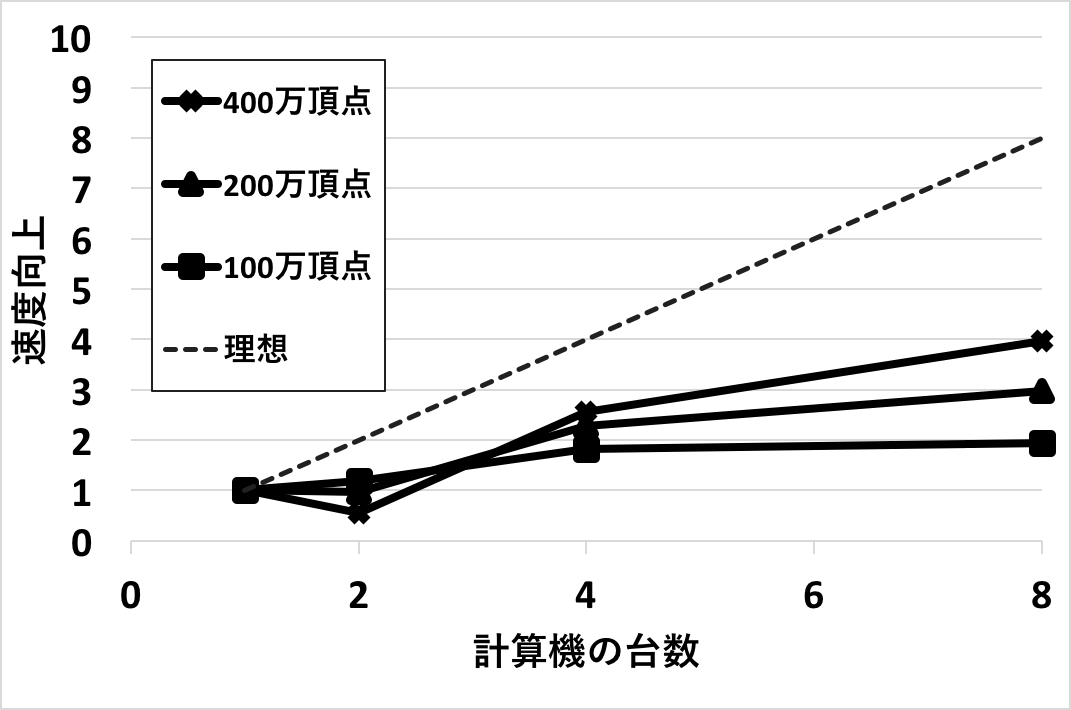
\includegraphics[width = 8cm]{kisuuPregel.png}
      \caption{Pregelコードの速度向上の様子}
    \end{center}
  \end{minipage}
\end{figure}

\begin{figure}[ht]
  \begin{minipage}{0.45\textwidth}
    \begin{center}
      \makeatletter
      \def\@captype{table}
      \makeatother
      \begin{tabular}{|c||c|c|c|c|}\hline
        計算機台数 & 1 & 2 & 4 & 8\\ \hline
        100万頂点 & 101.5 & 121.7 & 39.2 & 26.1\\ \hline
        200万頂点 & 210.0 & 404.3 & 75.6 & 39.1\\ \hline
        400万頂点 & 521.7 & 1555.5 & 200.8 & 71.4 \\ \hline
      \end{tabular}
      \caption{Fregelコードの実行時間(s)}
    \end{center}
  \end{minipage}
  \begin{minipage}{0.8\textwidth}
    \begin{center}
      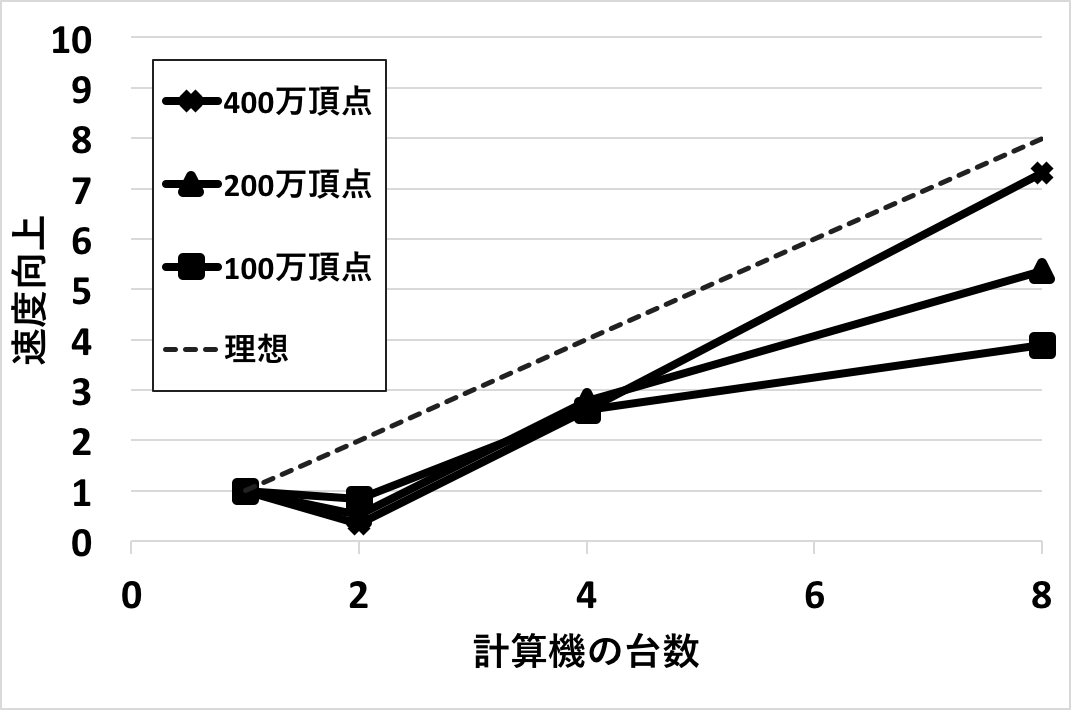
\includegraphics[width = 8cm]{kisuuFregel.png}
      \caption{Fregelコードの速度向上の様子}
    \end{center}
  \end{minipage}
\end{figure}

\newpage
図5.1,図5.2から,計算機の台数が4台以上の時には理想値には届いてないものの,速度が向上していることがわかる.
しかし,計算機の台数が2台の時は頂点数が増加するにつれて,速度が低下していることが確認できる.
理由として,二部グラフの頂点集合の分け方が原因であると考えられる.

本実験では,頂点IDの奇数,偶数により集合を区別している.
このプログラムにおいて,頂点間の通信は異なる集合に属する頂点間のみで行われる.
しかし,計算機2台で並列実行した際,片方の計算機に頂点IDが奇数の頂点集合,もう片方の計算機に偶数の頂点集合が割り当てられ,
計算機同士の通信量が増加したために速度が出なかったと思われる.
これを確かめるため,追加実験を行うこととした.

集合の区別方法を変更し,再度実験を行なった.
表5.4と表5.5に実行時間,図5.3と図5.4に速度向上の様子を示す.
この実験では,頂点IDが全頂点数の半分以下であるかどうかで頂点集合を区別している.

\begin{figure}[ht]
  \begin{minipage}{0.5\textwidth}
    \begin{center}
      \makeatletter
      \def\@captype{table}
      \makeatother
      \begin{tabular}{|c||c|c|c|c|}\hline
        計算機台数 & 1 & 2 & 4 & 8\\ \hline
        100万頂点 & 29.0 & 20.5 & 15.8 & 15.4 \\ \hline
        200万頂点 & 50.0 & 29.2 & 20.8 & 17.0 \\ \hline
        400万頂点 & 91.0 & 49.8 & 31.5 & 22.5 \\ \hline
      \end{tabular}
      \caption{Pregelコードの実行時間(s)}
    \end{center}
  \end{minipage}
  \begin{minipage}{0.7\textwidth}
    \begin{center}
      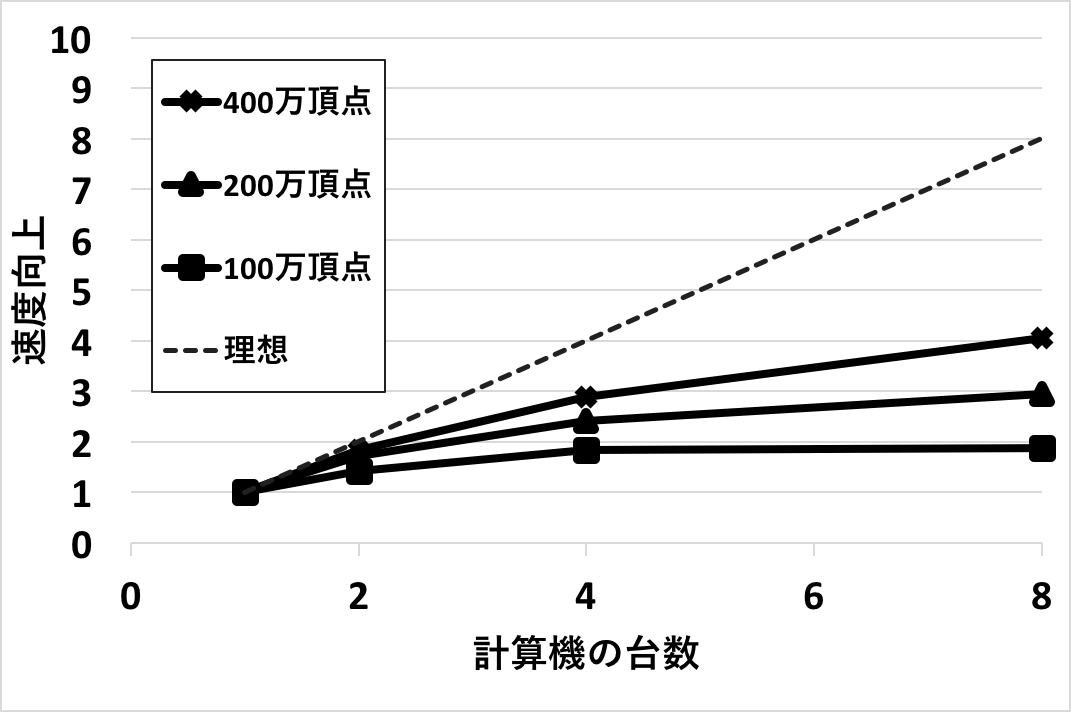
\includegraphics[width = 8cm]{hanPregel.png}
      \caption{Pregelコードの速度向上の様子}
    \end{center}
  \end{minipage}
\end{figure}

\begin{figure}[ht]
  \begin{minipage}{0.45\textwidth}
    \begin{center}
      \makeatletter
      \def\@captype{table}
      \makeatother
      \begin{tabular}{|c||c|c|c|c|}\hline
        計算機台数 & 1 & 2 & 4 & 8\\ \hline
        100万頂点 & 100.1 & 53.3 & 30.6 & 25.8 \\ \hline
        200万頂点 & 201.2 & 97.5 & 49.0 & 32.0 \\ \hline
        400万頂点 & 490.2 & 280.4 & 92.2 & 51.4  \\ \hline
      \end{tabular}
      \caption{Fregelコードの実行時間(s)}
    \end{center}
  \end{minipage}
  \begin{minipage}{0.8\textwidth}
    \begin{center}
      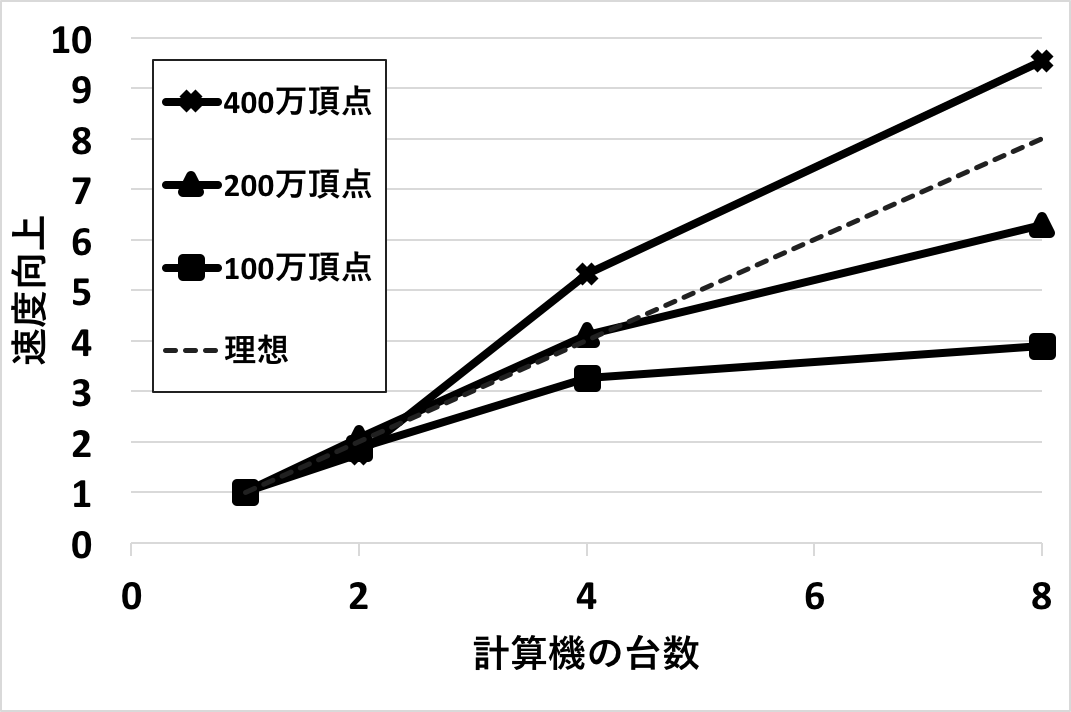
\includegraphics[width = 8cm]{hanFregel.png}
      \caption{Fregelコードの速度向上の様子}
    \end{center}
  \end{minipage}
\end{figure}
\newpage

図5.3,図5.4から,どの計算機の台数においても台数が増加するにつれて速度が向上していることがわかる.
また,頂点数が増加するにつれて速度向上が改善することが確認できる.
Fregelコードを400万頂点で実行した際には速度向上が理想以上に改善されているが,これはもはや1台で処理するにはグラフが大きすぎるからであり,大規模なグラフほど並列化の効果が顕著になることがわかる.
よって,本研究で拡張した機能を用いたグラフ計算においても,十分な並列性能が得られることがわかった.

\newpage

\chapter{まとめ}
本研究では,二部グラフマッチングを題材に,Fregelの機能の有用性の検証と機能拡張を行なった.
結果として,Fregelの拡張した機能を用いたグラフ計算においても十分な並列性能が確認できた.
また,集約関数randomの拡張により二部グラフマッチングを記述できたことで,少しの機能拡張によりグラフ計算を記述できるというFregelの記述性も確認された.

今後の課題として,次のようなことが考えられる.
まず,他のグラフ計算を記述する際に必要な機能がまだ不足しているため,Fregelの機能のさらなる拡張が必要となるだろう.
さらに,実際の実行時間を見てみるとFregelはPregelと比べて十分に早いとは言えない.
Fregelにおけるグラフ計算の速度向上も課題の一つである.

\newpage

\chapter*{謝辞}

本研究を進めるにあたり,指導教員の江本健斗准教授には様々なご指導を賜りました.
また,研究室の先輩,同級生には様々な助言を頂きました.
関わってくださった皆様に感謝の意を示します.

\newpage

\begin{thebibliography}{9}
  \bibitem{pregel}
  Grzegorz Malewicz, Matthew H. Austern, Aart J. C. Bik, James C. Dehnert, Ilan Horn, Naty Leiser, and Grzegorz Czajkowski.
  Pregel: a system for large-scale graph processing.
  In Proceedings of the ACM SIGMOD International Conference on Management of Data, pages 135-146, 2010.
  \bibitem{fregel}
  Kento Emoto, Kiminori Matsuzaki, Zhenjiang Hu, Akimasa Morihata, and Hideya Iwasaki.
  Think like a vertex, behave like a function! a functional DSL for vertex-centric big graph processing.
  In Proceedings of ICFP 2016, pages 200-213, 2016.
  \bibitem{giraph}
  Apache Giraph. https://giraph.apache.org/
  \bibitem{hadoop}
  Apache Hadoop. https://hadoop.apache.org/
  \bibitem{グラフ理論}
  惠羅博,土屋守正,『増補改訂版 グラフ理論』,産業図書,2011.
\end{thebibliography}

\end{document}
